\setlength\abovedisplayskip{0.4pt}
\setlength\belowdisplayskip{0.4pt}

\chapter{Introduction}

Microseconds after the big bang, the universe was filled with a hot, dense state of strongly interacting subnuclear particles \cite{Rafelski:2013obw}. There is evidence that this phase of matter, the quark gluon plasma (QGP), is reproduced in the high energy densities reached by ultra-relativistic heavy-ion collisions \cite{Arsene:2004fa}. Measurements at the Relativistic Heavy Ion Collider (RHIC) and the Large Hadron Collider (LHC) are consistent with the QGP having the sheer viscosity of a perfect fluid \cite{Long:796947}. In particular, at present the field of ultra-relativistic heavy-ion collisions focuses on measuring the QGP properties in detail. Heavy-ion initial state properties must be rigorously measured to distinguish between the effects of the QGP and of the inherent properties of the nucleus.

This thesis seeks to further knowledge of initial state phenomena in heavy-ion collisions by measuring the gluon distribution within the nucleus. In the context of coherent dijet photoproduction from ultra-peripheral collisions (UPC), the distribution of the so-called "elliptic" gluons is encoded in the angular correlation of the dijet\cite{Hagiwara:2016kam}. In UPCs all interactions between nuclei are from electromagnetic or electroweak processes \cite{Contreras:2015dqa}. Such photo-nuclear interactions are described via the equivalent photon approximation from the Weizacker-Williams formalism \cite{vonWeizsacker:1934sx,Williams:1934ad}, as discussed in chapter 2.

Before discussing the physics of ultra-peripheral collisions to that of UPC dijets, we will give an overview of the standard model of high energy physics, followed by an introduction to relativistic heavy-ion collisions and how these are connected to photon-induced interactions. 

\section{The Standard Model}

The Standard Model describes the fundamental particles of the universe in terms of fermions and bosons. Fermions are particles with half-integer spin, while bosons have integer-spin. Fermions must obey the Pauli Exclusion Principle: only one fermion at a time can occupy a given state. However, multiple bosons can simultaneously occupy a specific state \cite{Dyson:1967:SM}. Subnuclear particles -- protons and neutrons -- contain large numbers of both fermions and bosons. Fermions and bosons have different statistical properties. Fermi-Dirac statistics describe the energy distribution of fermions. Likewise, the boson energy distribution is described by Bose-Einstein statistics \cite{Huang_1987}. 

Among the fermions are the leptons, neutrinos, and quarks. The leptons consist of the electron, muon, and tau, as well as their anti-particles. The leptons are believed to be fundamental: high energy experiments have yet to observe internal lepton-structure. Neutrinos are weakly interacting particles detected primarily through the precise measuring of missing transverse energy in the products of particle collisions. Quarks are the constituent particles of baryons, which contain three valence quarks, and mesons, which contain two valence quarks. In addition to the valence quarks are the sea quarks, which appear and disappear as quark-antiquark pairs within hadrons. The hadrons are particles made of quarks and gluons. Gluons are particles that mediate the strong nuclear force; likewise, photons mediate the electromagnetic force, and weak-gauge bosons mediate the weak nuclear force. A fourth boson, the graviton, is expected to transmit the gravitational force, but this particle has not been observed \cite{Halzen:1984mc}. 

The behavior of fundamental particles is best described within the framework of quantum field theory (QTF). QFT defines a Lagrangian for fundamental particles. This Lagrangian then predicts the outcome of particle collisions. Different terms in the Lagrangian correspond to the various interactions between particles. The Standard Model Lagrangian, $\mathcal{L}_{Standard Model}$ can be broken down into three basic terms:	
\begin{equation}
\mathcal{L}_{Standard Model} = \mathcal{L}_{QED} + \mathcal{L}_{QCD} + \mathcal{L}_{Higgs} + ... ,  
\end{equation} 
where $\mathcal{L}_{QED}$ is the QED Lagrangian, $\mathcal{L}_{QCD}$ is the QCD Lagrangian, and $\mathcal{L}_{Higgs}$ is the Higgs Lagrangian. The QED and QCD Lagrangians will be the most important in what follows \cite{Halzen:1984mc}. 

The most accessible approach to quantum field theory is through the use of Feynman diagrams. First, one imagines an interaction between particles. Then, one draws this process into a Feynman diagram, which is essentially a pictorial representation of exchanges between particles. The Lagrangian can be interpreted into Feynman rules. These rules describe how the Feynman diagram translates into a calculation for the quantum mechanical amplitude of the process. The quantum mechanical amplitude, in turn, is proportional to the cross section of the process. This is important because, sense the cross-section is invariant between experiments, one can use it to effectively test for invariant quantities in the Lagrangian \cite{Peskin:1995ev}.

\section{Quantum electrodynamics}

Quantum electrodynamics (QED) is a theory of electromagnetic interactions in terms of relativistic quantum field theory. The QED Lagrangian is
\begin{equation}
{\mathcal {L}}={\bar {\psi }}(i\gamma ^{\mu }D_{\mu }-m)\psi -{\frac {1}{4}}F_{\mu \nu }F^{\mu \nu },
\end{equation} 
where $\psi$ is spin-$\frac{1}{2}$ field, $\gamma^\mu$ are the Dirac matrices, $D_\mu$ is the gauge covariant derivative, $m$ is the electron mass, and $F_{\mu\upsilon}$ is the electromagnetic field tensor \cite{Peskin:1995ev}.

QED addresses three specific processes: photon motion, electron motion, and the emission or absorption of a photon by an electron. First a Lagrangian is established based on Maxwell's laws and quantum mechanics. The photon constitutes a spin-1 solution to the differential equations derived from the QED Lagrangian. Likewise, electrons are described, at non-relativistic scales, by the is Schr\"{o}dinger equation, and at relativistic scales by the Dirac equation. There are three processes allowed by QED: the translation of an electron, the translation of a photon, and the scattering of a photon off an electron \cite{Griffiths:2008zz}. 

The QED coupling constant, $\alpha_{em}$, is approximately 1/137 at perturbative scales \cite{Bouchendira:2010es}. In general, the cross section of a given process is proportional to the $(\alpha_{em})^n$ where $n$ is the number of vertices in the Feynman diagram. The more complex the Feynman diagram, the smaller its cross section. However, at small scales, i.e. non-perturbative momentum transfers $Q^2$, the coupling constant increases. $\alpha_{QED}$ is defined as
\begin{equation}
\alpha_{QED}(Q^2) = \frac{ \alpha_{em}}{(1 - \frac{\alpha_{em}}{3\pi})\mathrm{ln}(\frac{Q^2}{m^2}) },
\end{equation}
where $\alpha_{QED}(Q^2)$ is the QED coupling constant at high $Q^2$, and $m$ is the electron mass \cite{Abbiendi:2005rx}. High values of $Q^2$ are non-perturbative because, at small scales and high momentum, the fluctuation of photons into electron-positron pairs begins to saturate. Particle and anti-particle pairs can pop into exist, persist a short time, and then annihilate so long as quantum numbers are conserved. 

\section{Quantum chromodynamics}

The parton model, first proposed by Richard Feynman, posits that hadrons in general, and nucleons in specific, are made of more fundamental constituent particles which may or may not be the quarks implied by the SU(3) symmetry. In addition to the quarks, the partons also include any field quanta associated with nuclear forces. In time, these field quanta are named "gluons".

The quarks are a family of fermions that compose the baryons and the mesons. Baryons consist of three quarks in a color neutral state, while mesons consist two quarks in a color neutral state. "Color" in this context refers to the six kinds of strongly-interacting charge available to quarks: red and anti-red, blue and anti-blue, and green and anti-green. Color charge has no relation to optical phenomena, but provides a useful analogy for the stable combinations of quarks. The net color-charge of a baryon or meson is colorless. By way of analogy, a red quark, green quark, and blue quark can together form a hadron, in the way that conventional red, green, and blue can together form white \cite{Brock:1993sz}. 

Gluons are the QCD analogues of the photons in QED. Gluons are spin-1 and massless, but unlike photons, which do not carry electromagnetic charge, gluons carry strongly-interacting charge \cite{Wilczek:2000ih}. The QCD Lagrangian, which encodes the interactions of gluons and quarks, is
\begin{equation}
{\mathcal {L}}_{\mathrm {QCD} }={\bar {\psi }}_{i}\left(i(\gamma ^{\mu }D_{\mu })_{ij}-m\,\delta _{ij}\right)\psi _{j}-{\frac {1}{4}}G_{\mu \nu }^{a}G_{a}^{\mu \nu },
\end{equation}
where $m$ now represents the quark mass, the $\delta_{ij}$ is the delta function and $G_{\mu \nu }^{a}$ is gluon field tensor,  
\begin{equation}
\displaystyle G_{\mu \nu }^{a}=\partial _{\mu }{\mathcal {A}}_{\nu }^{a}-\partial _{\nu }{\mathcal {A}}_{\mu }^{a}+gf^{abc}{\mathcal {A}}_{\mu }^{b}{\mathcal {A}}_{\nu }^{c}.
\end{equation}
The SU(3) group of the quarks is indexed as $i,j,...$; the adjoint SU(3) group, for the gluons, is indexed $a,b,c$. ${\mathcal {A}}_{\nu }^{a}$ is the gluon field, $f^{abc}$ are the SU(3) structure constants, and $g$ is the strong coupling \cite{Schafer:2005ff}. 

Unlike QED, the QCD coupling increases with distance \cite{Bethke:2006ac}. Figure \ref{fig:runningQCDCoupling} shows the running of the QCD coupling with $Q^2$:
\begin{equation}
\alpha_{QCD}(Q^2) = \frac{4 \pi }{(11 - \frac{2}{3}n_f)\mathrm{ln}(\frac{Q^2}{\Lambda^2_{QCD}}) } ,
\end{equation}
where $n_f$ is the number of quark flavors, $Q^2$ is the momentum transfer, and  $\Lambda^2_{QCD}$ is the mass scale \cite{Deur:2016tte}. The running coupling has the practical consequence of the strong-interactions being stronger in high momentum transfer collisions. The direct results of the running QCD coupling include the dual phenomena of asymptotic freedom and color confinement. At large distances, string tension describes the binding force of the quarks. At short distances, however, Coulomb-like interactions dominate \cite{Bjorken:1968dy}. The QCD coupling constant can be measured via the cross-section of inelastic proton-proton collisions, and also the cross section of electron-positrons into triple jets \cite{Thomson:2013zua}. 
\begin{figure}[h!]
\begin{centering}
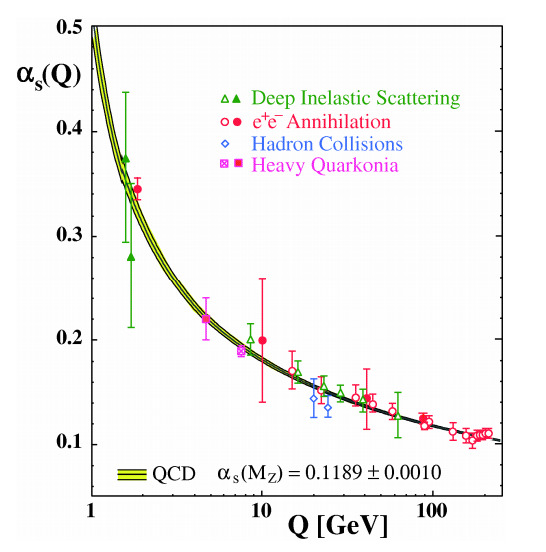
\includegraphics[width=4in]{Chapter1/importfigs/qcd_coupling_bethke.png}
\par\end{centering}
\caption{QCD coupling constant as a function of $Q^2$ \cite{Bethke:2006ac}. \label{fig:runningQCDCoupling}}
\end{figure}

\section{Deep inelastic scattering}

At the turn of the century, Ernst Rutherford probed the gold atom by bombarding a gold sheet with alpha-particles. The angular distribution of the scattered alpha-particles demonstrates that the mass of the atom is concentrated in a small volume, i.e, the atom is mostly empty space. Further experiments revealed that the atomic nuclei consisted of separate positively and neutrally charged particles: protons and neutrons. Scattering experiments are the basic tool for exploring the nucleus. In particular, DIS commonly refers to the scattering of a lepton off hadrons. For example, experiments at HERA focused on electron-proton collisions. In these collisions, the electron was used as a source of photons and neutrinos. When these particles scatter off the proton, the dependence of the collision cross section, on momentum transfer and scattering angle of the source electron, reflects the structure of the proton. DIS experiments provided the first evidence of two phenomena: the parton model and Bjorken-scaling. 

The momentum transferred, $Q^2$, is an important quantity for characterizing DIS measurements. In addition to $Q^2$, Bjorken-$x$ is necessary to describe the nuclear phase space. Bjorken-x represents the momentum fraction of partons. In the context of lepton-proton scattering, it was observed that at high momentum transfers the structure functions of the proton were functions of $Q^2/\upsilon$, where $Q^2$ is the squared four-momentum of the virtual photon emitted by the electron, and $\upsilon$ is the energy lost by the electron in the collision \cite{Bjorken:1968dy}. 

"Scaling" is an interpretation of the data from DIS. First proposed by James Bjorken, scaling is reflected in the incoherence of photon-proton interactions at photon energies above 1 $GeV/c$ \cite{Bjorken:1982qr}. Predictions from perturbative QCD are in good agreement with DIS data from HERA, as seen in figure \ref{fig:qcdBjorkenX} \cite{Shimizu:2009fc}. In this graph the Bjorken-$x$ momentum fraction is designated $x$, and $\sigma_r$ represents the $F_2$ structure function, and $Q^2$ is the transferred momentum from the electron to the proton. The order of magnitude of $\sigma_r$ set by the Bjorken-x.

\begin{figure}[h!]
\begin{centering}
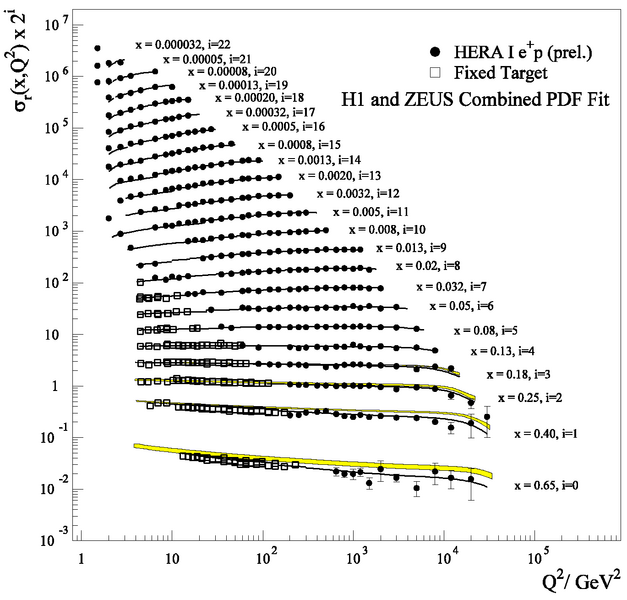
\includegraphics[width=4in]{Chapter1/importfigs/scholarpedia_bjorken_x_qcdExp.png}
\par\end{centering}
\caption{Collision cross section as a function of Bjorken-$x$, with data compared to HERA-PDF calculations \cite{Shimizu:2009fc}. \label{fig:qcdBjorkenX}}
\end{figure}

At the small scales probed by high energy photons, the decreasing QCD coupling causes quarks and gluons to interact weakly. This phenomena is called "asymptotic freedom". Because gluons themselves carry color charge, the gluons about a quark tend to have an anti-screening behavior: the gluon color adds to the quark color, increasing the net color charge of the area. At smaller distances to a quark, then, there are fewer and fewer gluons augmenting the color interaction.

\section{PDFs}

QCD describes the interaction between quarks and gluons, but within a nucleon the calculations are too complicated to solve for the behavior of each individual parton. Theorists employ the factorisation theorem to use data from DIS experiments to make predictions. The factorisation theorem is discussed in greater detail later in section 2.3. Parton distribution functions (PDFs) are a method of encoding data from DIS experiments in the form of probability density. PDFs give the probability of finding a species of parton with given momentum fraction, $x$, and a given squared energy scale, $Q^2$ \cite{Martin:2009iq,Eskola:2008ca,Pumplin:2002vw,cmsJpPP}.

In electron-proton deep inelastic scattering, the electron interacts with the proton electromagnetically by the emission of a virtual photon. This virtual photon has a four momentum $q$ and a virtuality $Q^2 = - q^2$. When virtuality is low, the virtual photon is approximately "real"; these quasi-photons are discussed in greater detail in chapter 2. The virtual photon, originating from the electron, interacts with a parton and changes its initial momentum fraction, $x$. The $Q^2$ of the probing virtual photon and Bjorken-x of interacting parton are determined from the collision products. The data can be used to fill out a probability density, $F_i(x, Q^2)$, of finding a parton species $i$ at a given momentum fraction $x$ with a probe of virtuality $Q^2$.

The HERA results show that the parton density rapidly increases as the momentum fraction decreases. Conservation of momentum demands that the splintering of partons must eventually cease. The specific saturation point, where recombination begins dominates, is a characteristic of high energy gluons within a hadron.

\begin{figure}[h!]
\begin{centering}
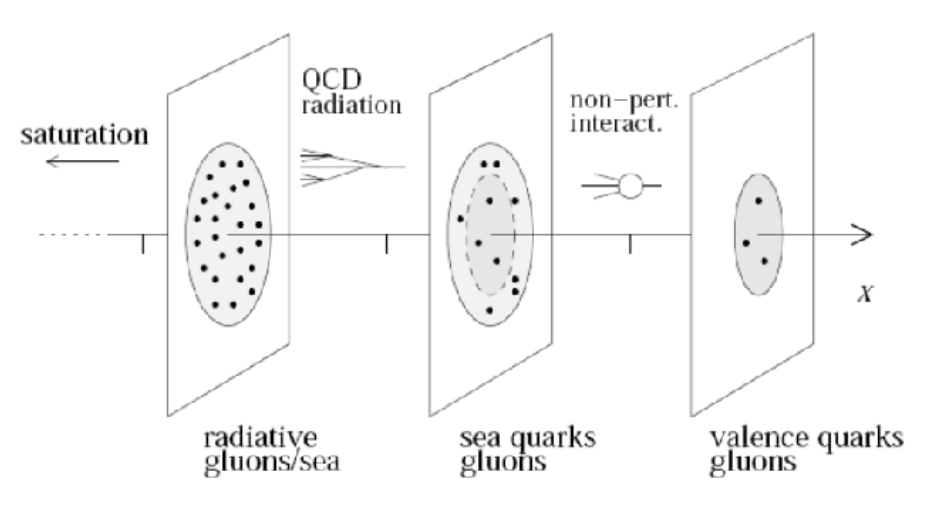
\includegraphics[width=7in]{Chapter1/importfigs/imaging_the_nucleon_upc_dijets_pres.png}
\par\end{centering}
\caption{Subnuclear tomography \cite{Accardi:2011mz}. \label{fig:nuclImag}}
\end{figure}

Figure \ref{fig:nuclImag} shows an illustration of how the nucleus appears at varying momentum fractions \cite{Accardi:2011mz}. Because of confinement and asymptotic freedom the hadronic bound states are too complex for an analytic solution. Furthermore, collider experiment data requires a quantitative interpretation to be useful. The gap between QCD and heavy-ion data is bridged using the parton model, which considers hadrons as composed of quarks and gluons. Parton density functions (PDFs) model the longitudinal momentum distribution of the partons. PDFs are supplemented by transverse momentum distributions (TMDs) and generalized parton distributions (GPDs). In addition to transverse momentum, GPDs describe the transverse spatial distribution. TMDs and GPDs are derived from the final state particles of a collision.

\section{Quark gluon plasma}

From 1980's to 2000's, the Super Proton Synchrotron (SPS) and the Relativistic Heavy Ion Collider (RHIC) performed heavy ion experiments to study the possibility of deconfined plasma in a high parton density medium \cite{spsHI,ags2rhic,etaOvSinit}. These experiments confirmed the developing model of the QCD phase space; see Figure \ref{fig:QCDPhase} \cite{Bhalerao:1695331}. Essentially, quark matter organizes itself differently depending on temperature and baryon density. At low energies, quark matter exists in bound states: the hadrons. However, in the high energy limit, quarks and gluons take the form of a strongly interacting plasma: QGP. The QGP represents the extreme case of asymptotic freedom; the QCD coupling constant becomes small enough that quarks and gluons no longer behave as bound states. There are two ways of achieving the high energies necessary to form QGP. High baryon densities cause the quarks of separate hadrons to interact at small distances where asymptotic freedom takes effect. It is not currently possible to achive these densities in laboratory experiments, though this state is thought to occur in neutron stars. By contrast, particle colliders like the LHC increase the energy density by colliding heavy-ions at ultra-relativistic velocities. The high temperature environment produces QGP. The early universe, mere milliseconds after the Big Bang, is thought to have existed as QGP \cite{Hands:2001ve}.


\begin{figure}[h!]
\begin{centering}
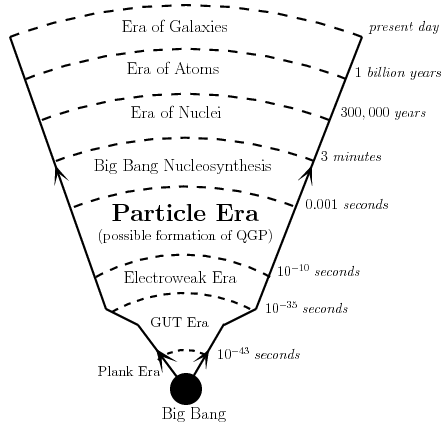
\includegraphics[width=5in]{Chapter1/importfigs/fig_bb_timeline.png}
\par\end{centering}
\caption{Pictorial time-line of the Universe, showing phase transitions \cite{Bandyopadhyay:2017wip}. \label{fig:history}}
\end{figure}

Figure \ref{fig:history} is a simplified cosmological timeline. In the first hundred or so microseconds after the Big Bang, the universe was small, dense, and highly energetic \cite{Bandyopadhyay:2017wip}. The energy density of the early universe would have been in excess of 1 $GeV/(fm)^3$. Note that 1 $GeV/(fm)^3$ is the energy density at which QGP is thought to form. The universe cools and hadrons form out of the quarks and gluons. The protons and neutrons condense into nuclei. The positively charged nuclei gather negatively charged electrons, forming the atoms that in cosmic time become stars \cite{Witten:1984rs}.

\begin{figure}[h!]
\begin{centering}
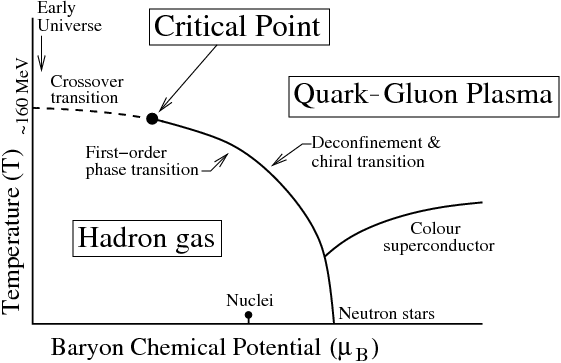
\includegraphics[width=4in]{Chapter1/importfigs/byr13.png}
\par\end{centering}
\caption{QCD phase diagram showing the temperature $T$ as a function of baryon chemical potential $\mu_B$. Different phases such as the critical point, QGP, and hadron gas are seen \cite{Bhalerao:1695331}. \label{fig:QCDPhase}}
\end{figure}

There are a number of experimental signatures of QGP formation. Thermal physics understands phase transitions as occuring at specific temperatures and densities. At the boundary between two phases, one can define a critical point at which there is a discontinuous change in the behavior of observables. For the SPS and RHIC heavy-ion programs the main observables were charm suppression and strangeness enhancement, elliptic flow, and jet quenching \cite{Gyulassy:1990ye,Matsui:1986dk,Margetis:2000sv}.

The QGP is thought to suppress the production of $J\psi$ mesons in heavy-ion collisions. Figure \ref{fig:jpsiSupp} shows the suppression of $J/\psi$ with respect to Drell-Yan scattering in Pb-Pb collisions at SPS \cite{spsHI}.
\begin{figure}[h!]
\begin{centering}
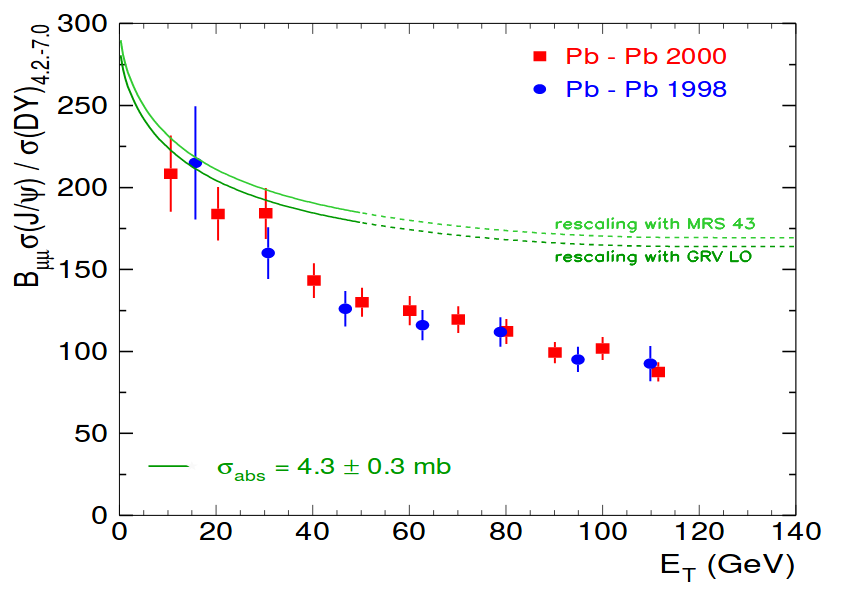
\includegraphics[width=4in]{Chapter1/importfigs/jpsiSupp.png}
\par\end{centering}
\caption{$J/\psi$ suppression as a function of transverse energy $E_T$ in Pb-Pb collisions at SPS. Data from different periods are shown and compared to theories that do not incorporate QGP \cite{spsHI}. \label{fig:jpsiSupp}}
\end{figure}

In addition, the predicted viscosity of QGP would cause elliptic flow in the overlap region of heavy-ion collisions \cite{phobosFlow}. At RHIC, it was demonstrated that heavy-ion collisions can produce a state of hadronic matter, often referred to as "the medium", that exhibits elliptic flow. The angular correlations of the final state particles, produced by heavy-ion collisions, were analyzed and shown to be consistent with the medium flowing as a nearly ideal fluid \cite{Chatrchyan:2013nka}. "Ideal fluid" refers to how the high temperature nuclear medium can be modelled by hydrodynamic equations in which the shear viscosity is extremely low \cite{Karsch:2000kv}.

As the QGP is a perfect fluid, the initial state properties of the heavy-ion will propagate through the collision and have a significant effect on the final state particles. The angular distribution of final state particles can be modelled using Fourier series,
\begin{equation}
 1+\sum^{\infty}_{n=1}2v_{n}\mathrm{cos}\left[n\left(\phi-\Psi\right)\right],
\end{equation}
where $n$ is the order of the Fourier expansion, $v_n$ is the Fourier coefficient, $\phi$ is the azimuthal angle, and $\Psi$ is the event-plane angle. The 2nd order term, $v_2$, is referred to as "elliptic flow" and is predicted to quantify the pressure gradient of the overlap-region in the heavy-ion collision. Figure \ref{fig:overlap} is an illustration of the overlap region of a heavy-ion collision. Because the pressure gradient is higher for the short axis than for the long axis, the nuclear medium in the overlap region will flow outward along the short axis, and this is reflected in the alignment of the tracks in the direction of the flow \cite{Abelev:2012ola,Ollitrault:1992bk,Sorensen:2009cz,Bhalerao:2003yq,Borghini:2001zr,Ackermann:2000tr,Borghini:2004ke}. 

\begin{figure}[h!]
\begin{centering}
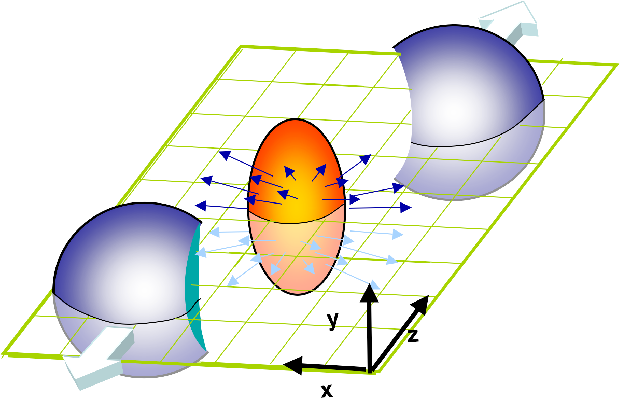
\includegraphics[width=4in]{Chapter1/importfigs/elliptic_flow_3D_medium.png}
\par\end{centering}
\caption{Heavy-ion overlap region, showing the elliptic flow produced. \label{fig:overlap}}
\end{figure}
A highly viscous medium will resist deformation such that the shape of the overlap region, i.e. its ellipticity, will not necessarily carry over to the final-state tracks. However, because the QGP medium is a nearly ideal liquid, the elliptic correlation of the final-state should arise from that of the inital-state. The RHIC result emphasizes the great importance of a precisely understood heavy-ion initial state. Figure \ref{fig:hiFlow} compares the $v_2$ elliptic flow results from various heavy-ion experiments \cite{spsHI}.
\begin{figure}[h!]
\begin{centering}
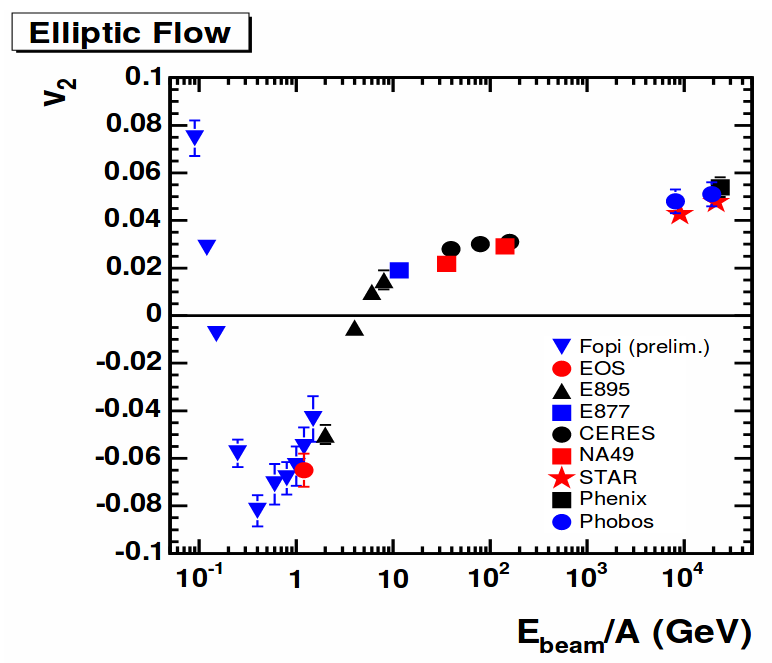
\includegraphics[width=4in]{Chapter1/importfigs/elliptic_flow.png}
\par\end{centering}
\caption{$v_2$ as a function of collision energy for various heavy ion experiments \cite{spsHI}. \label{fig:hiFlow}}
\end{figure}

Figure \ref{fig:exampleStarKine} shows $v_2$ measurements from $\sqrt{S_{NN}}=130$ GeV $Au+Au$ collisions by the STAR Collaboration. The hydrodymanic limit is thought to describe the behavior of QGP. At lower centrality the hydrodynamic limit is in good agreement with data, but the overestimation of data at high centrality is consistent with the rapid thermalization of QGP shortly after collision. The linear $p_T$ dependence of elliptic flow implies that the expansion is enhanced in the collision plane \cite{Ackermann:200tr}. 

\begin{figure}%
    \centering
    \subfloat[]{{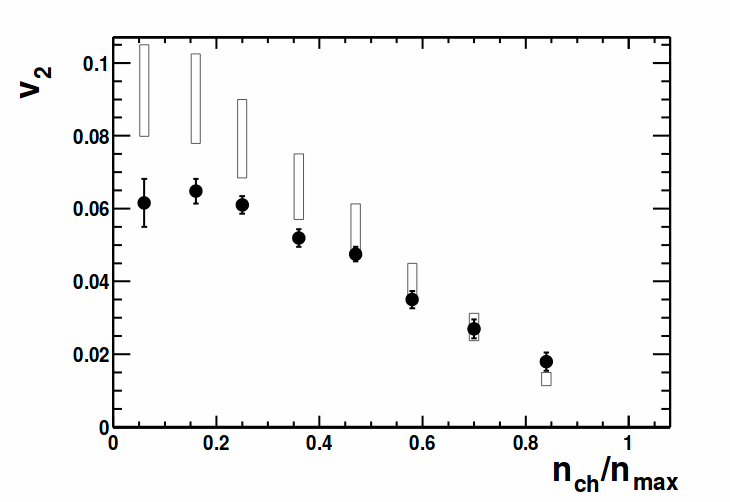
\includegraphics[width=6cm]{Chapter1/importfigs/star_130_fig3.png} }}%
    \qquad
    \subfloat[]{{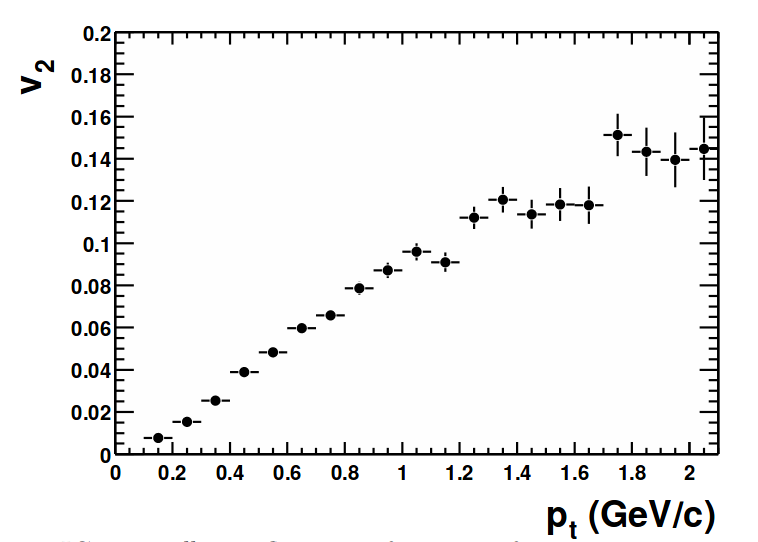
\includegraphics[width=6cm]{Chapter1/importfigs/star_130_fig4.png} }}%
    \caption{STAR $Au+Au$ at $\sqrt{s_{NN}}=130$ GeV: (a)$v_2$ as a function of centrality with hydrodynamic calculations (empty rectangles) and data (black dots); (b)$v_2$ as a function of $p_T$ \cite{Ackermann:2000tr}.}%
    \label{fig:exampleStarKine}%
\end{figure}

Figure \ref{fig:exampleRidge} displays one of the most striking phenomena associated with heavy-ion flow: "the Ridge". There is a distinct pattern to the two-particle correlations of high $p_T$ tracks in heavy-ion collisions. Notice that compared to pPb data the PbPb ridge is narrower, implying a stronger correlation and more pronounced elliptic flow \cite{Chatrchyan:2013nka}. 

\begin{figure}%
    \centering
    \subfloat[]{{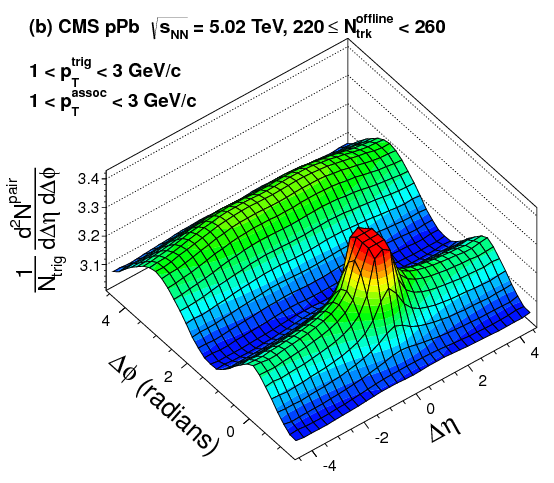
\includegraphics[width=6cm]{Chapter1/importfigs/corr2D_pPbNew_pt0-0_nmin220_nmax260_20130206.png} }}%
    \qquad
    \subfloat[]{{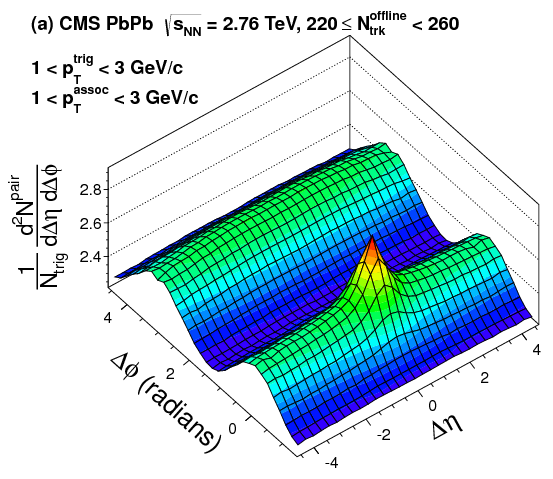
\includegraphics[width=6cm]{Chapter1/importfigs/corr2D_PbPb_pt0-0_nmin220_nmax260_20130325.png} }}%
    \caption{CMS (a) pPb and (b) PbPb, angular correlations \cite{Chatrchyan:2013nka}}%
    \label{fig:exampleRidge}%
\end{figure}

The phase transitions from a hot, dense medium to stable hadrons are seen in heavy-ion collisions, as illustrated by figure \ref{fig:historyHI} \cite{Wang:2012jua}. The y-axis represents time, and the x-axis represents the longitudinal separation of the ions. Notice that after the ions cross, there is a "cascade" during which the partons take on thermal energy until reaching a critical temperature for QGP formation. The hadron gas passes through two temperature "freeze-out". When particles stop forming the chemical freeze-out temperature. These particles stop exchanging kinetic energy after cooling beyond the "kinetic freeze-out" \cite{bjEdense}.

\begin{figure}[h!]
\begin{centering}
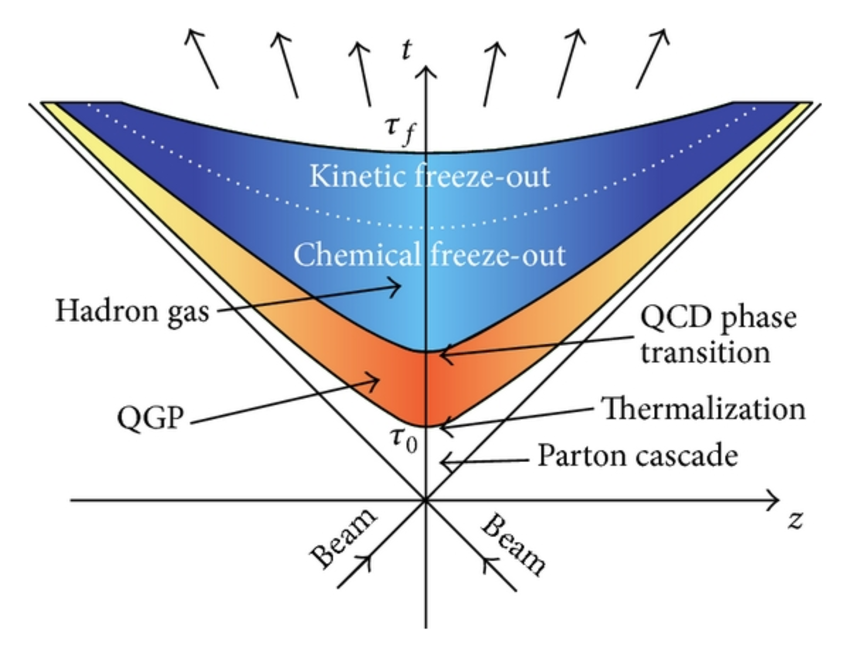
\includegraphics[width=5in]{Chapter1/importfigs/The-space-time-evolution-of-heavy-ion-collision-The-figure-is-taken-from-28.png}
\par\end{centering}
\caption{Space-time diagram of a heavy-ion collision \cite{Wang:2012jua}.\label{fig:historyHI}}
\end{figure}

Lastly, hadronic jets would interact strongly with the QGP; therefore, dijets will have significant energy imbalance depending on the multiple interactions of the components jet with the QGP. All of these cases require a good understanding the heavy-ion initial state as a basis for comparison \cite{Vogt:1998kna}. 

The Large Hadron Collider (LHC) stands at the forefront of high energy nuclear physics research. The LHC is capable of reaching heavy-ion collision energies of up to 7 TeV per nucleon-nucleon, which is sufficient energy for a QGP to be formed and to last long enough to measure its properties \cite{Roland:2014jsa,Frankfurt:2005mc,Vogt:2002ve}.